\documentclass[10.5pt, oneside, twocolumn]{article}   	% use "amsart" instead of "article" for AMSLaTeX format
\usepackage[margin=0.7in]{geometry}                		% See geometry.pdf to learn the layout options. There are lots.
\geometry{letterpaper}                   		% ... or a4paper or a5paper or ... 

\usepackage[parfill]{parskip}
\usepackage{graphicx}		
\graphicspath{ {Figures/} }							
\usepackage{amssymb}
\usepackage[english]{babel}
\usepackage{csquotes}
\usepackage{amsmath}
\usepackage{booktabs}

\usepackage[backend=biber,sorting=none]{biblatex}
\bibliography{deepiv_gwas}


\title{Deep IV with Whole-Omics Data to Identify Novel Carcinogenesis-Mediating Pathways \\
	\vspace{3mm}
	\large Category: Health / Genomics}
\author{
	Jack Andraka\\ 
	\texttt{jandraka@stanford.edu}
	\and
	Billy Ferguson\\
	\texttt{billyf@stanford.edu}
	\and
	Charlie Walker\\
	\texttt{cwalker4@stanford.edu}
}
\date{}							% Activate to display a given date or no date

\begin{document}
\maketitle
\section{Introduction}
Breast cancer accounts for over 25\% of cancer diagnoses and 15\% of cancer-related deaths in women.\cite{torre2016global} Ten percent of women with breast cancer have a family history of the disease; women with one premenopausal first-degree relative with breast cancer are at 3.3-fold greater risk than women without a family history, demonstrating that there is a significant genetic contribution to breast cancer risk. To identify genetic factors associated with breast cancer, early studies employed linkage analysis and positional cloning in families with a familial history of breast cancer to discover highly penetrant susceptibility genes such as BRCA1\&2.\cite{joosse2012brca1} Although these initial studies could explain about 20\% of the familial risk of breast cancer,\cite{thompson2004genetic} they provided little insight into the role of genetics in nonfamilial breast cancer. \\

More recently, genome-wide association studies (GWAS) have identified over 80 loci significantly associated with sporadic breast cancer. However, these variants collectively only explain 16\% of breast cancer heritability.\cite{skol2016genetics} The inability of GWAS to identify a greater proportion of the genetic risk stems from many factors, including genotyping platform limitations in interrogating rare variation (primarily due to the running of several thousand to several million t-tests simultaneously). This is in contrast with the current hypothesis of genetic architecture that posits many gene variants acting in tandem to produce a phenotypic trait, each with small effect size.\cite{de2010predicting} The GWAS study design is also plagued by confoundedness, despite the development of many sophisticated statistical techniques to deal with complicated interactions. Simple prediction and correlation setups in breast cancer studies fail to account for this confoundedness (gene expression results in cancerous growth and cancerous growth impacts gene expression). \\

Instrumental variables (IV) have proven to be an adept statistical method for addressing these issues of confoundedness. As shown in Figure 1, IV uses an exogenous instrument $z$ to identify direct causal relationships between some policy variable $p$ on outcome $y$ (a relationship confounded by latent effects $e$). In the case of genetics studies, Mendelian randomization of genetic variants offers a promising instrument for estimating causal effects of gene expression on cellular phenotype, in this case if the cell is cancerous or not.\cite{burgess2017dissecting} In this manner, it is possible to identify low-signal, rare variants that would typically not appear in GWAS analyses, thus providing a more comprehensive mapping of the transciptome of a cell to carcinogenesis. \\

Traditional IV experimental designs suffer from the limitation that they require a strong prior understanding of the data generating process (DGP), and are limited in accounting for complex interactions between covariates. Neural networks offer a solution to this limitation, due to their ability to model complicated interactions between genes that are both near and distal.\cite{cheng2011recurrent} This project uses the DeepIV framework  to characterize the causal effect of gene expression on carcinogenesis in breast cancer using random, simple nucleotide variants (SNVs). 

\section{Algorithm}
\subsection{Overview}
We implement the method described in ``Deep IV: A Flexible Approach for Counterfactual Prediction'' to identify the effect of a policy variable $p$ on outcome $y$ in the presence of confoundedness.\cite{hartford2017deep} Instrumental variables (IV) are a well-developed tool for remedying endogeneity, but require a strong prior understanding of the data generating process and are not well equipped to deal with a large number of covariates. Deep IV promises to marry the best qualities of DNNs and IV, and we believe GWAS are a prime use case. \\

To perform IV analysis one needs to find an exogenous variable that affects the outcome variable only through the endogenous covariate of interest. More specifically, the instrument \emph{z} must be conditionally independent of the error (Figure 1).\\

\begin{figure}[h]
	\caption{Generalized Deep IV}
	\centering
	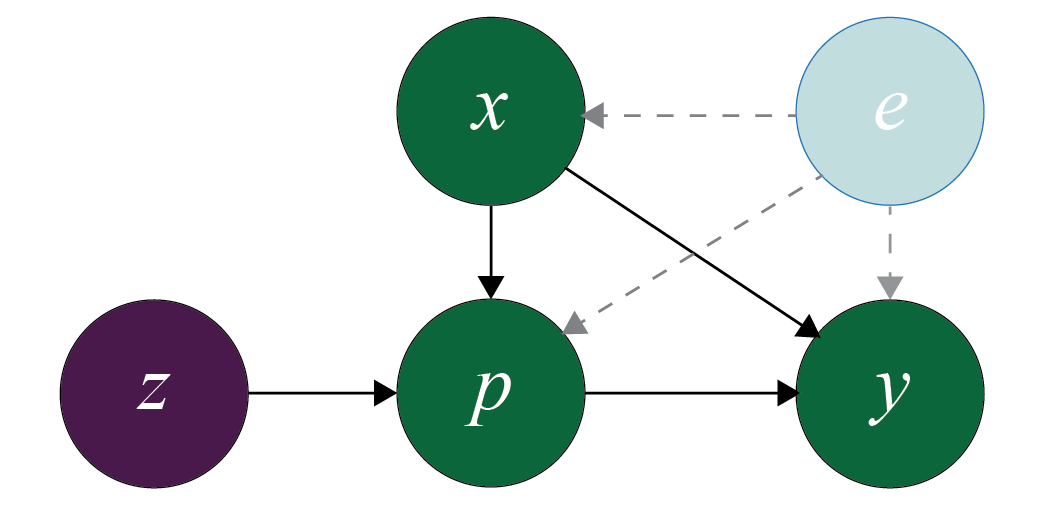
\includegraphics[width=0.4\textwidth]{Figure_1.png}
\end{figure}

Traditional IV can be estimated through a procedure called two-stage least squares (2SLS): in the first stage you regress your endogenous variable of interest, $p$, on the exogenous instrument, $z$, to create a predicted $\hat{p}$ constructed only with the exogenous variation of $z$. In the second stage, you regress your outcome variable, $y$, on the predicted $\hat{p}$ from the first stage.\footnote{Chapter 4 of Angrist and Pischke's \emph{Mostly Harmless Econometrics: an Empiricist's Companion}\cite{angrist2008mostly} provides a good introduction to instrumental variables.} To adapt this procedure for the DeepIV method, we replace the two-stage least squares with two-stage multilayer perceptrons. We call the first stage our \emph{policy network} and the second our \emph{response network}.\\

\section{Simulation}
\subsection{Motivation and Design}
As a proof-of-concept, we evaluate our approach on simulated data, testing DeepIV's ability to recover an underlying causal relationship in a low-dimensional domain. We compared our DeepIV architecture to a single-stage feed-forward network with the same architecture as our  DeepIV \emph{response} stage. 

\subsection{Simulated Data}
Our simulation models a DGP similar to that described in Section 2. For ease of explanation, we ground our simulation in a typical real-world IV application: estimating the effect of price on sales of some product (say, hotel bookings). We begin by assuming seven customer types, $s \in \{1,...,7\}$ which each exhibit different levels of price sensitivity. Customer price sensitivity varies according to a complex non-linear function of time.
\begin{gather*}
\psi_t = 2\big((t-5)^4/600 + \textrm{exp}\big[-4(t-5)^2\big] + t/10 - 2 \big)\\
t \sim \textrm{unif}(0,10)
\end{gather*}
Prices are a function of observed variable $t$ and some instrument $z$, on the basis that the hotel chooses their price to move with average price sensitivity. In the hotel example, the high demand resulting from some unobserved confounding variable (e.g. a nearby conference) breaks the conditional independence between our policy variable $p$ (price) and the latent effects $e$. We model this by generating our errors $e$ with parameter $\rho$ that denotes the correlation between $p$ and $e$; in other words, it reflects the extent of endogeneity in our population model. Our outcome variable $y$ (sales) is then generated as:
\begin{gather*}
y = 100 + (100 + p)s\psi_t - 2p + e \\
p = 25 + (z + 3)\psi_t + v \\
z, v \sim \mathcal{N}(0,1) \\
e \sim \mathcal{N}(\rho v, 1 - \rho^2)
\end{gather*}
The causal relationship we wish to uncover is $h(t, s, p) = (10 + p)s\psi_t - 2p$, but the correlation between the error $e$ and $p$ in our population model violates the unconfoundedness assumption necessary for causal interpretation. \\

Since we have our ground truth causal relationship, we evaluate our model by first generating features $[t, s, p]$, but then change $p$ to a fixed grid of price values $p'$. This allows us to compare our predicted sales, $\hat{h}$ against the ground truth $h$. 

\subsection{Model Architectures}\

The policy and response networks in our simulations below have three hidden layers with 128, 64, and 32 hidden units respectively. The policy network takes in the exogenous $z$ and control variables $x$ as input to predict $p$ using tanh activation functions for each layer and a Mixture of Gaussian output with 10 components. The predicted $\hat{p}$ from the policy network and $x$ are then fed into the response network to yield predictions $\hat{y}$. The response network uses ReLU activation functions for the three hidden layers and linear activation for the output. \\

Both networks use Adam Optimization with learning rate $=0.001$, $\beta_1 = 0.9$, $\beta_2 = 0.999$, and $\epsilon = 1e-08$. For training we use L2 weight decay with penalty parameter $0.001$, a dropout rate of $\textrm{min}(1000/(1000+n); 0.5)$, $(1.5 \times 10^6/n)$ epochs, and batch size $100$. 

\subsection{Results} 
\begin{figure}[h]
	\caption{Causal Performance (n=1000)}
	\centering
	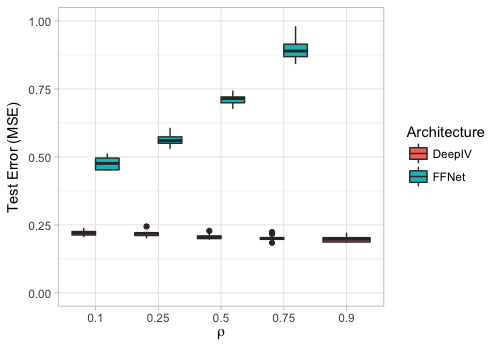
\includegraphics[width=0.4\textwidth]{perf_small.png}
\end{figure}

\begin{figure}[h]
	\caption{Causal Performance (n=10,000)}
	\centering
	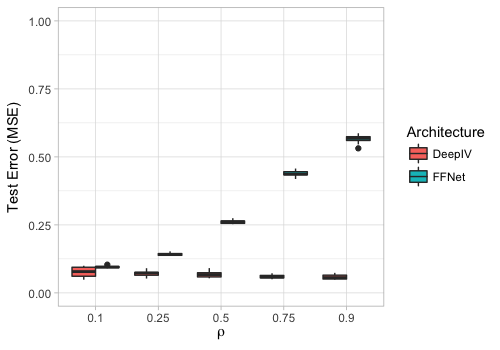
\includegraphics[width=0.4\textwidth]{perf_big.png}
\end{figure}

Figures 2 and 3 summarize the results of our simulations for two different $n$, giving out-of-sample MSE as we vary the level of endogeneity in our DGP. Each model was fit on 10 random samples from the DGP for each $\rho$ and sample size. The performance of the DeepIV architecture was largely unaffected by the increase in $\rho$, reflecting the resilience of this architecture to confounding latent variables. On the other hand, the Feed-Forward Network did a poor job of recovering the true counterfactual function we were testing with this simulation.\footnote{Note that this model would have performed well if we had been testing its ability to estimate $h(t, s, p) + \mathbb{E}[e | p]$, i.e. if we were not trying to make counterfactual predictions.}

\section{Breast Cancer}

\subsection{Data}
We use whole-genome and whole-transcriptome data from the Genotype-Tissue Expression (GTEx) project \cite{gtex2015genotype} and The Cancer Genome Atlas (TCGA)\cite{tomczak2015cancer}. The GTEx dataset includes 11,688 samples that are non-cancerous with matched whole-genome and whole-transcriptome data. The TCGA dataset includes 978 breast cancer samples with matched whole-genome and whole transcriptome data. 

Due to the highly unique property of genetic mutations, the instrument space would be too large if genetic mutations were categorized by base pair loci for each unique mutation (i.e. a specific mutation typically only occurs in a single person in the dataset). To address this, we employed the degree of mutation of a gene for an individual as our instrumental variable, which is defined as the number of mutations an individual had on a specific gene, measured for all sequenced genes. Transcriptome data was defined as abundance of an mRNA transcript, measured by transcripts per million transcripts (concentration). \\

There are 13,980 genes and 53,196 transcripts measured in our combined data. To make network training computationally tractable, we reduced the transcript space to 2,344 transcripts of genes that were utilized in a previous transcriptome analysis project in breast cancer carcinogenesis. The resulting instrument dataset was sparse, with each healthy individual having an average of 3 mutations and each cancerous individual having an average of 77.34 mutations. However, this degree of sparsity is characteristic of large SNP mutation datasets and is not expected to negatively impact the performance of our model. We used a 80:15:15 split for train, validate, and test (respectively), resulting in a train set with $n = 8866$, and validation and test sets with $n = 1900$.

\subsection{Network Architecture}
For the first stage of our DeepIV framework we predict 2,344 gene expression levels from genetic variants, normalizing observed gene expression for each mRNA. We experimented with a variety of model architectures (number of layers and nodes per layer in a Feed-Forward Network), and subsequently used a grid search over relevant hyperparameters to optimize our performance on the validation set. A sample of our candidate models for the first stage is given in Table 1; our chosen architecture was three fully connected layers with 200 hidden units, tanh activation functions, a learning rate of 1e-3, and a hefty dropout rate of 50\%. We used Adam optimization with parameters as specified in the seminal paper\cite{kingma2014adam} and a batch size of one hundred.

The first stage reached its minimum validation error within a few epochs. Even with extensive regularization and a relatively simple architecture our validation error quickly began to climb, reflecting the fact that our data is relatively wide. Below we show the training and validation MSE for five model specifications. We characterize each model by: layers, learning rate, L2, dropout rate, activation function. 

\begin{table}[h]
\centering
\caption{First Stage Models}
\label{my-label}
\begin{tabular}{@{}lllll@{}}
\toprule
Model & Train & Validation &  \\ \midrule
{[}100,100,100{]}, 1e-3, 0, 0, tanh         & .974           & .976    \\
{[}200, 100, 50{]}, 1e-3, 0, 0.4, tanh      & .806           & 1.085   \\
{[}200, 200, 200{]}, 1e-3, 0, 0.5, tanh*    & .983           & .975  \\
{[}200, 200, 200{]}, 1e-3, 0, 0, tanh       & .974           & .976     \\
{[}200, 200, 200{]}, 1e-3, 1e-4, 0, tanh    & 1.002          & .993     
\end{tabular}
\end{table}

Using our preferred model for the first stage, we feed the training data through the trained first stage, and use these predicted gene expression levels as the training data for the second stage. 

In designing the second stage we again explored a variety of architectures and compared validation error over a grid of hyperparameters. Since our outcome is now binary, we use a sigmoid output and binary cross-entropy loss. A grid search over our hyperparameters yielded a model with a learning rate of 3e-5, dropout rate of 0.1, and no L2 regularization. Again, we used Adam optimization and a batch size of one hundred. The training and validation binary cross-entropy loss for a sample of five candidate specifications can be seen below. 

\begin{table}[h]
\centering
\caption{First Stage Models}
\label{my-label}
\begin{tabular}{@{}lllll@{}}
\toprule
Model & Train & Validation &  \\ \midrule
{[}50, 50{]}, 1e-5, 0, 0, sigmoid         & .019           & .019    \\
{[}100, 50{]}, 3e-5, 1e-4, 0, tanh      & .036          & .038   \\
{[}100, 50{]}, 3e-5, 0, 0.1, tanh*    & .013          & .014  \\
{[}100, 50{]}, 1e-5, 0, 0, tanh       & .014         & .017     \\
{[}100, 50, 10{]}, 1e-5, 0, 0, sigmoid    & .044         & .046    
\end{tabular}
\end{table}\textit{}

\subsection{Results}
Using our preferred models for both the first and second stage we achieve a misclassification rate of 0.5 percent; the ROC curve (Figure 4) for our final model confirms that we do a near-perfect job at predicting whether or not a cell is cancerous as we vary our classification threshold (our default  is 50\%). 


\begin{figure}[h!]
	\caption{ROC Curve for Final Predictions}
	\centering
	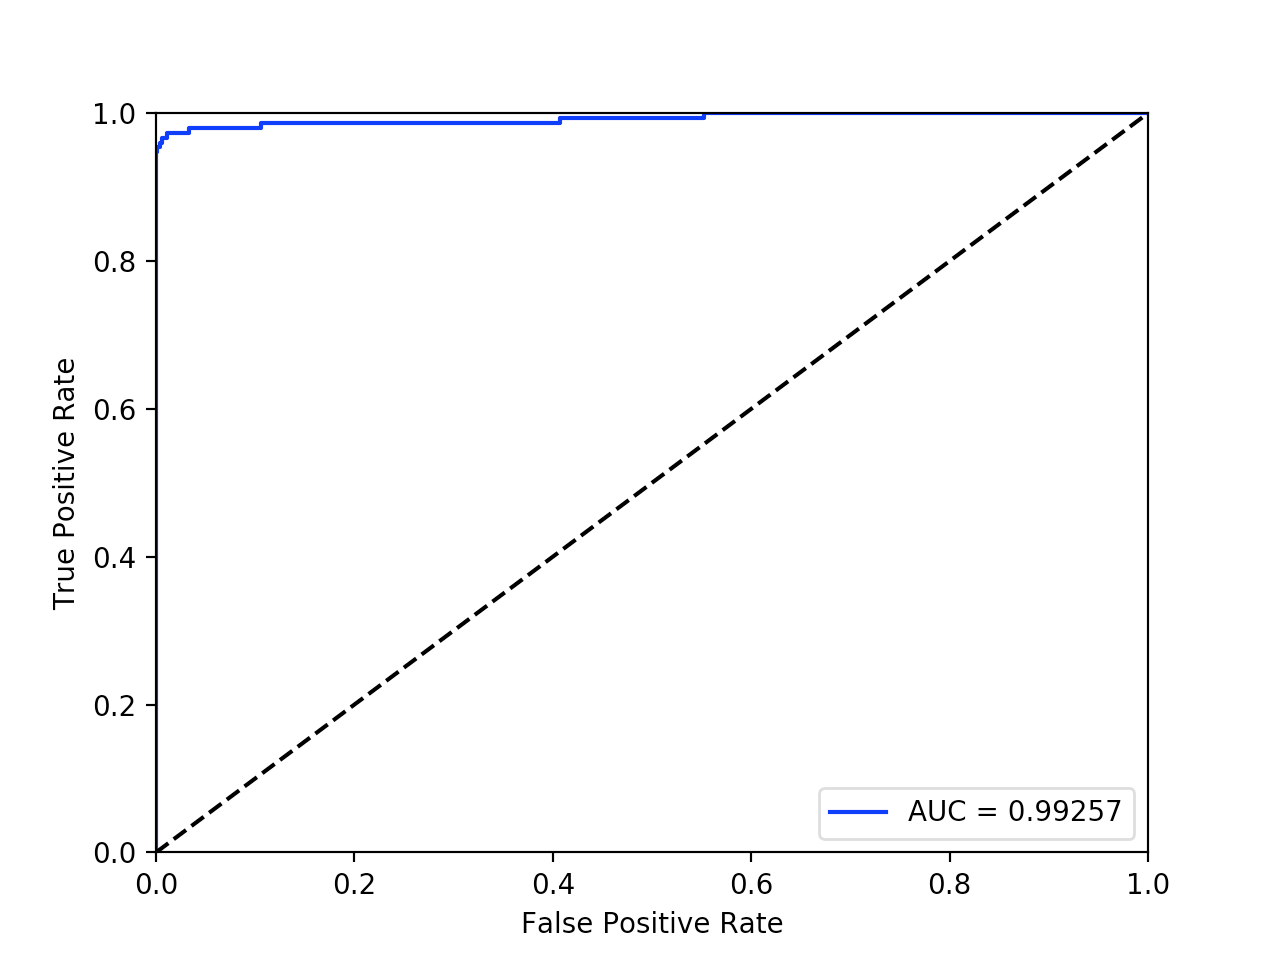
\includegraphics[width=0.4\textwidth]{roc_curve.png}
\end{figure}

While we are pleased with the low error rate we were able to achieve with the DeepIV method, the true comparative advantage comes not in predictive accuracy, but in interpretability. By removing the confounded relationship between gene expression and cancer in the first stage, the second stage can be understood in a causal framework. Running a set of gene expression levels through the second stage does not yield the predicted outcome (i.e. predictions in the presence of endogeneity), but rather the outcome \textit{caused} by the mRNA expression. 

We can now exploit the second stage to simulate controlled lab experiments. To rigorously understand how gene expression levels influence cancer, scientists have been forced to carefully (and expensively) underexpress or overexpress genes in a lab. This is the only scientific way to understand the relationship since any observational data occurring in nature is plagued by the endogenous relationship between the variable of interest and the outcome. However, the trained second stage of the DeepIV model simulates lab experiments since it has insured unconfoundedness. We can thus choose whatever gene expression is of interest to us, run it through the second stage, and understand how those particular gene expression levels cause cancer. 

To understand and discover the causal effect of gene expression on cancer, we generated 100,000 observations from a multivariate Gaussian distribution for the 2,344 different mRNA, using our training data to estimate the covariance matrix. We then fed this data through the second stage to yield causal outcomes. Because our second stage network captures the true causal relationship irrespective of endogeneity (Section 3), we could then use classical statistical learning techniques to uncover (and represent) the causal relationships between gene expressions and carcinogenesis using our simulated data.

We first ran an L1-penalized logistic regression to yield a sparse vector of mRNAs with the most significant causal impact on carcinogensis, choosing the penalty parameter by 5-fold cross-validation. The largest 10 coefficients (in absolute value) are given in Table 3. We also trained a classification decision tree with an information gain criterion to model interactions between mRNAs, 4 levels of which are shown in Figure 5.

These simulation experiments yielded a myriad of new candidate genes involved in carcinogenesis that have not been fully characterized, and in some cases explored, for breast cancer. The most significant gene was PSMG1, which was identified as having the largest discriminating ability between healthy and cancerous cells by the decision tree, being used as the classifier in both of the first two splits, as well as having the second largest coefficient (in absolute terms) in the logistic regression. Both analyses indicated that underexpression of PSMG1 increases carcinogenesis; this aligns well with PSMG1’s role as a chaperone protein in the assembly of the 20S proteasome, which is essential in the degradation of mutated and misfolded proteins\cite{vidal1998identification}. \\

\begin{table}[h]
\centering
\caption{Top Lasso Coefficients}
\begin{tabular}{@{}ll@{}}
\toprule
mRNA ID            & Coefficient         \\ \midrule
ENSG00000121621 & -2.253  \\
ENSG00000183527 & -1.381 \\
ENSG00000100842 & 1.263  \\
ENSG00000141873 & -1.148 \\
ENSG00000162738 & 0.937   \\
ENSG00000155330 & -0.934 \\
ENSG00000197557 & -0.926 \\
ENSG00000128581 & -0.888 \\
ENSG00000116704 & -0.767 \\
ENSG00000213463 & -0.683 \\ \bottomrule
\end{tabular}
\end{table}

The decision tree also identified that overexpression of the TRIM29 protein, a transcriptional regulatory factor involved in carcinogenesis \cite{sho2011trim29}, and underexpression of the PERP protein, a regulator of the p53 pathway (a tumor suppressor pathway)\cite{attardi2000perp}, increase carcinogenesis, which agrees with previous characterization of these protein’s function as described in the literature. Although PSMG1, TRIM29, and PERP have all been investigated for carcinogenesis involvement prior to this project, none of these proteins have been robustly characterized in breast cancer specifically, presenting an exciting avenue for future investigations into breast cancer carcinogenesis and therapeutic targets. The logistic regression both reiterated the significance of the PSMG1 protein, as well as identified nine new candidate proteins for carcinogenesis regulation. In particular, the SLC39A3\cite{kelleher2009zip3}, VANGL2\cite{andre2012wnt}, c16orf87\cite{tan2013functional}, and SLC35D1\cite{hiraoka2007nucleotide} proteins have never been investigated in breast cancer carcinogenesis, with their mechanisms for carcinogenesis still being unknown. Further analysis of these proteins using decision tree analysis will elucidate the associated carcinogenesis-mediating interactions and present potential routes for further characterization of breast cancer carcinogenesis. 

\begin{figure}[!hb]
	\caption{Truncated Decision Tree}
	\centering
	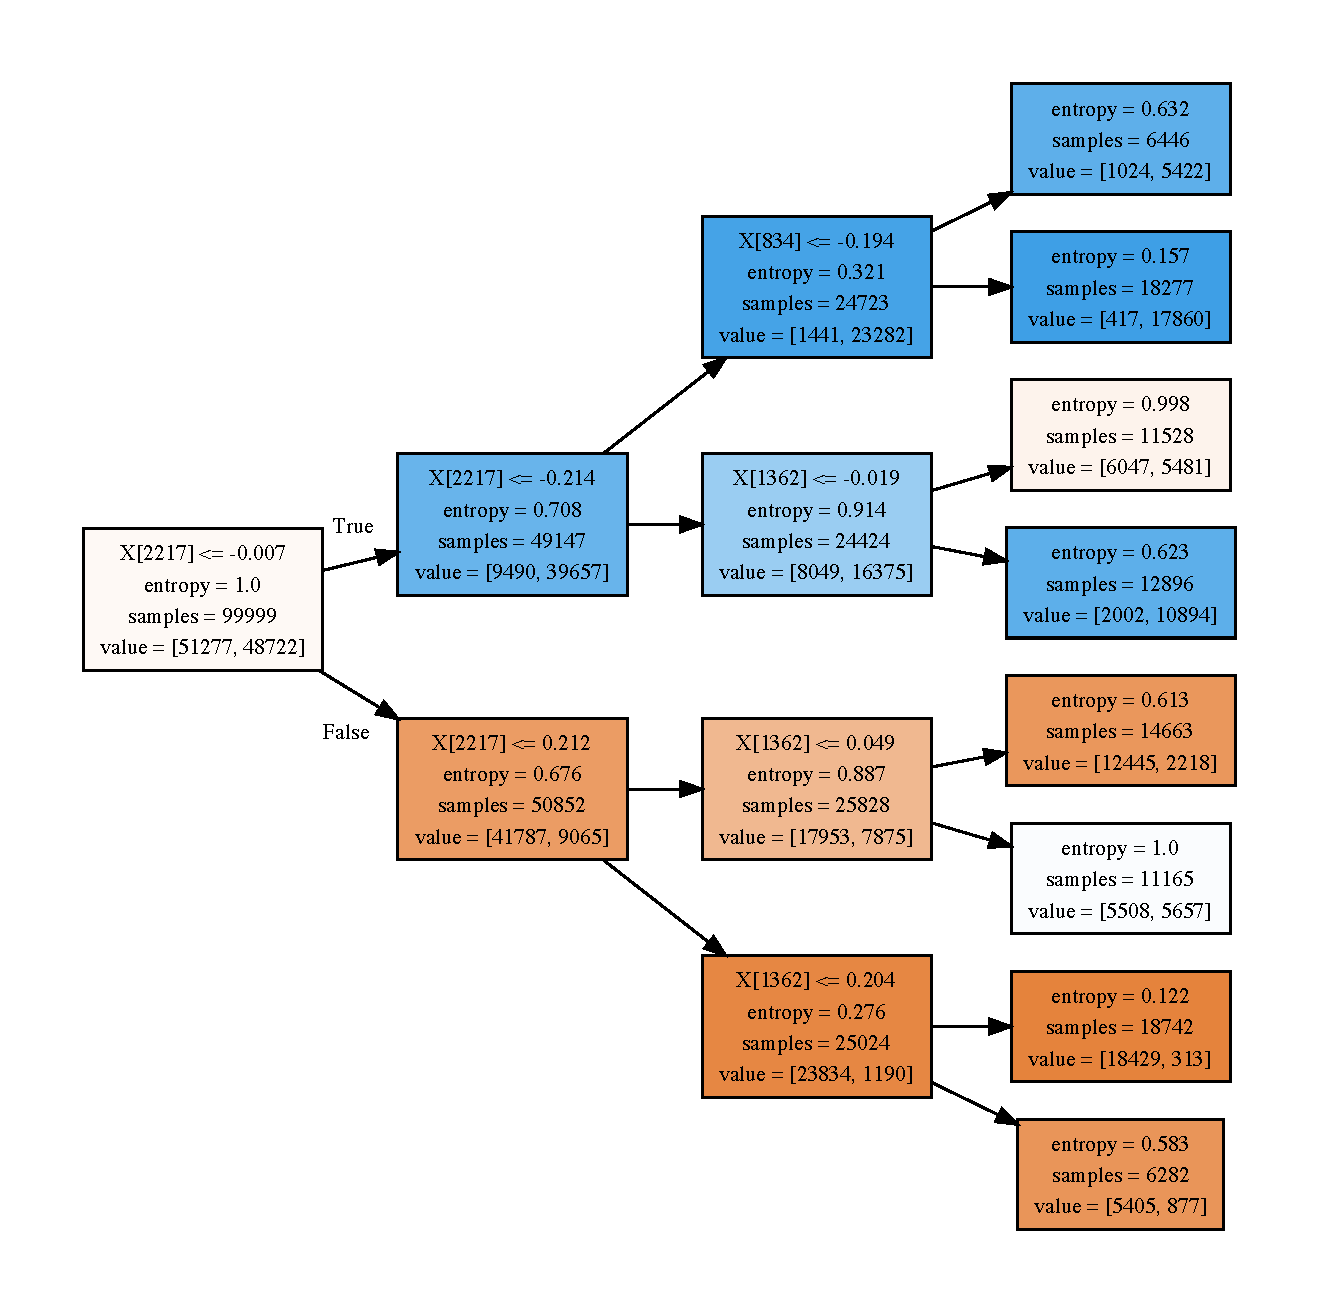
\includegraphics[width=0.4\textwidth]{graph_3.pdf}
\end{figure}


\section{Future Work}
Although we discovered a number of  transcripts that are influential in mediating carcinogenesis in breast tissue as well as quantifying their causative effect on carcinogenesis, we cannot a priori validate our findings without some positive control or wet-lab experiments. This would consist of manual up- and down-regulation of the identified genes to reduce the abundance of the corresponding transcripts followed by monitoring for carcinogenesis behavior (i.e. measuring mutant p53 levels). Additionally, this study suffers from batch effect, due to all healthy samples coming from the GTEx dataset and all cancerous samples coming from the TCGA dataset. In order to develop a more robust model, we have partnered with Dr. Assimes of the Stanford School of Medicine to work with NIH data that does not exhibit batch effects, as well as increase the sample size and utilize the complete transcriptome space.


\section{Contributions}
\begin{itemize}
\item Jack Andraka: data access and cleaning, biology literature review, hyperparameter tuning, interpreting results\\
\item Billy Ferguson: data cleaning, model architecture, simulation, hyperparameter tuning\\
\item Charlie Walker: data cleaning, model architecture, simulation, hyperparameter tuning
\end{itemize}

\section{Code}
The code for this project is available at \url{https://github.com/cwalker4/deepiv-gwas}.

\section{Acknowledgements}
We'd like to thank Surag Nair for his advice and guidance throughout this project, Professor Susan Athey for pointing us towards DeepIV, Professor Bejerano for his early-stage advice on data, Professor Tim Assimes for his mentorship as we move forward with this project, and the entire teaching team of CS230 for a fantastic quarter!

%\onecolumn

\printbibliography



\end{document}  